\documentclass{standalone}
\usepackage{tikz}
\begin{document}
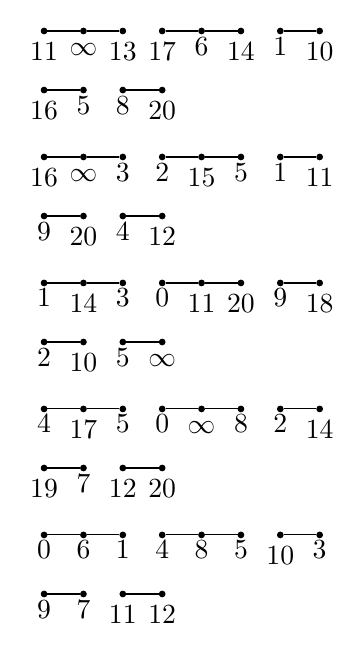
\begin{tikzpicture}[every node/.style={draw, circle, fill=black, minimum size=2pt, inner sep=0pt}]
\node[fill=black, label=below:{\color{black}$11$}] (G1N11) at (3.70,7.80) {};
\node[fill=black, label=below:{\color{black}$\infty$}] (G1Ninf) at (4.20,7.80) {};
\node[fill=black, label=below:{\color{black}$13$}] (G1N13) at (4.70,7.80) {};
\node[fill=black, label=below:{\color{black}$17$}] (G1N17) at (5.20,7.80) {};
\node[fill=black, label=below:{\color{black}$6$}] (G1N6) at (5.70,7.80) {};
\node[fill=black, label=below:{\color{black}$14$}] (G1N14) at (6.20,7.80) {};
\node[fill=black, label=below:{\color{black}$1$}] (G1N1) at (6.70,7.80) {};
\node[fill=black, label=below:{\color{black}$10$}] (G1N10) at (7.20,7.80) {};
\node[fill=black, label=below:{\color{black}$16$}] (G1N16) at (3.70,7.05) {};
\node[fill=black, label=below:{\color{black}$5$}] (G1N5) at (4.20,7.05) {};
\node[fill=black, label=below:{\color{black}$8$}] (G1N8) at (4.70,7.05) {};
\node[fill=black, label=below:{\color{black}$20$}] (G1N20) at (5.20,7.05) {};
\draw (G1N11) -- (G1Ninf);
\draw (G1Ninf) -- (G1N13);
\draw (G1N14) -- (G1N6);
\draw (G1N6) -- (G1N17);
\draw (G1N1) -- (G1N10);
\draw (G1N5) -- (G1N16);
\draw (G1N8) -- (G1N20);
\node[fill=black, label=below:{\color{black}$16$}] (G2N16) at (3.70,6.20) {};
\node[fill=black, label=below:{\color{black}$\infty$}] (G2Ninf) at (4.20,6.20) {};
\node[fill=black, label=below:{\color{black}$3$}] (G2N3) at (4.70,6.20) {};
\node[fill=black, label=below:{\color{black}$2$}] (G2N2) at (5.20,6.20) {};
\node[fill=black, label=below:{\color{black}$15$}] (G2N15) at (5.70,6.20) {};
\node[fill=black, label=below:{\color{black}$5$}] (G2N5) at (6.20,6.20) {};
\node[fill=black, label=below:{\color{black}$1$}] (G2N1) at (6.70,6.20) {};
\node[fill=black, label=below:{\color{black}$11$}] (G2N11) at (7.20,6.20) {};
\node[fill=black, label=below:{\color{black}$9$}] (G2N9) at (3.70,5.45) {};
\node[fill=black, label=below:{\color{black}$20$}] (G2N20) at (4.20,5.45) {};
\node[fill=black, label=below:{\color{black}$4$}] (G2N4) at (4.70,5.45) {};
\node[fill=black, label=below:{\color{black}$12$}] (G2N12) at (5.20,5.45) {};
\draw (G2N16) -- (G2Ninf);
\draw (G2Ninf) -- (G2N3);
\draw (G2N2) -- (G2N15);
\draw (G2N15) -- (G2N5);
\draw (G2N1) -- (G2N11);
\draw (G2N9) -- (G2N20);
\draw (G2N4) -- (G2N12);
\node[fill=black, label=below:{\color{black}$1$}] (G3N1) at (3.70,4.60) {};
\node[fill=black, label=below:{\color{black}$14$}] (G3N14) at (4.20,4.60) {};
\node[fill=black, label=below:{\color{black}$3$}] (G3N3) at (4.70,4.60) {};
\node[fill=black, label=below:{\color{black}$0$}] (G3N0) at (5.20,4.60) {};
\node[fill=black, label=below:{\color{black}$11$}] (G3N11) at (5.70,4.60) {};
\node[fill=black, label=below:{\color{black}$20$}] (G3N20) at (6.20,4.60) {};
\node[fill=black, label=below:{\color{black}$9$}] (G3N9) at (6.70,4.60) {};
\node[fill=black, label=below:{\color{black}$18$}] (G3N18) at (7.20,4.60) {};
\node[fill=black, label=below:{\color{black}$2$}] (G3N2) at (3.70,3.85) {};
\node[fill=black, label=below:{\color{black}$10$}] (G3N10) at (4.20,3.85) {};
\node[fill=black, label=below:{\color{black}$5$}] (G3N5) at (4.70,3.85) {};
\node[fill=black, label=below:{\color{black}$\infty$}] (G3Ninf) at (5.20,3.85) {};
\draw (G3N1) -- (G3N14);
\draw (G3N14) -- (G3N3);
\draw (G3N0) -- (G3N11);
\draw (G3N11) -- (G3N20);
\draw (G3N9) -- (G3N18);
\draw (G3N2) -- (G3N10);
\draw (G3N5) -- (G3Ninf);
\node[fill=black, label=below:{\color{black}$4$}] (G4N4) at (3.70,3.00) {};
\node[fill=black, label=below:{\color{black}$17$}] (G4N17) at (4.20,3.00) {};
\node[fill=black, label=below:{\color{black}$5$}] (G4N5) at (4.70,3.00) {};
\node[fill=black, label=below:{\color{black}$0$}] (G4N0) at (5.20,3.00) {};
\node[fill=black, label=below:{\color{black}$\infty$}] (G4Ninf) at (5.70,3.00) {};
\node[fill=black, label=below:{\color{black}$8$}] (G4N8) at (6.20,3.00) {};
\node[fill=black, label=below:{\color{black}$2$}] (G4N2) at (6.70,3.00) {};
\node[fill=black, label=below:{\color{black}$14$}] (G4N14) at (7.20,3.00) {};
\node[fill=black, label=below:{\color{black}$19$}] (G4N19) at (3.70,2.25) {};
\node[fill=black, label=below:{\color{black}$7$}] (G4N7) at (4.20,2.25) {};
\node[fill=black, label=below:{\color{black}$12$}] (G4N12) at (4.70,2.25) {};
\node[fill=black, label=below:{\color{black}$20$}] (G4N20) at (5.20,2.25) {};
\draw (G4N4) -- (G4N17);
\draw (G4N17) -- (G4N5);
\draw (G4N0) -- (G4Ninf);
\draw (G4Ninf) -- (G4N8);
\draw (G4N2) -- (G4N14);
\draw (G4N7) -- (G4N19);
\draw (G4N12) -- (G4N20);
\node[fill=black, label=below:{\color{black}$0$}] (G5N0) at (3.70,1.40) {};
\node[fill=black, label=below:{\color{black}$6$}] (G5N6) at (4.20,1.40) {};
\node[fill=black, label=below:{\color{black}$1$}] (G5N1) at (4.70,1.40) {};
\node[fill=black, label=below:{\color{black}$4$}] (G5N4) at (5.20,1.40) {};
\node[fill=black, label=below:{\color{black}$8$}] (G5N8) at (5.70,1.40) {};
\node[fill=black, label=below:{\color{black}$5$}] (G5N5) at (6.20,1.40) {};
\node[fill=black, label=below:{\color{black}$10$}] (G5N10) at (6.70,1.40) {};
\node[fill=black, label=below:{\color{black}$3$}] (G5N3) at (7.20,1.40) {};
\node[fill=black, label=below:{\color{black}$9$}] (G5N9) at (3.70,0.65) {};
\node[fill=black, label=below:{\color{black}$7$}] (G5N7) at (4.20,0.65) {};
\node[fill=black, label=below:{\color{black}$11$}] (G5N11) at (4.70,0.65) {};
\node[fill=black, label=below:{\color{black}$12$}] (G5N12) at (5.20,0.65) {};
\draw (G5N0) -- (G5N6);
\draw (G5N6) -- (G5N1);
\draw (G5N4) -- (G5N8);
\draw (G5N8) -- (G5N5);
\draw (G5N3) -- (G5N10);
\draw (G5N7) -- (G5N9);
\draw (G5N11) -- (G5N12);
\end{tikzpicture}
\end{document}
